%width of the three types of plots
\newcommand{\plotwidth}{0.63\linewidth}
\newcommand{\cfinderwidth}{0.96\linewidth}
\newcommand{\otherplotswidth}{0.76\linewidth}

As in the last section, we first discuss our results for the non-overlapping case followed by 
the ones for the overlapping case.

\subsection{Non-overlapping communities}
Figures~\ref{fig:no_iter_no_overlap}, \ref{fig:iter_no_overlap}, and~\ref{fig:compare_iter_no_overlap}
show the plots that we obtained for non-overlapping communities. Figure~\ref{fig:no_iter_no_overlap}
shows tests for the non-iterative method of our algorithm with 5, 10, 15, and 20$\%$ seed nodes per 
community. The first observation here is that anything less than 10$\%$ seed nodes per community 
will probably not give good results. With a seed node percentage of 10$\%$ or more and 
a mixing factor of at most~$0.4$ we acheive an NMI above $0.9$ and can compete with \textit{Infomap}, 
which was deemed to be one the best performing algorithms on the LFR benchmark~\cite{LF09}. 
Above a mixing factor of $0.4$, our algorithm has a worse performance than \textit{Infomap} 
which, curiously enough, achieves an NMI of around 1 till a mixing factor of around 
$0.6$ after which its performance drops steeply. The drop in the pereformance of our algorithm 
begins earlier but is not as steep.\texttt{having a comparative plot for Infomap would be nice at this point.}

Figure~\ref{fig:iter_no_overlap} shows the results for the iterative approach of 
our algorithm in the non-overlapping case. When compared with the non-iterative approach, 
one can see that even after ten iterations there is a significant improvement in 
performance (See Figure~\ref{fig:compare_iter_no_overlap}). As can be seen, typically 
with 6$\%$ seed nodes per community we obtain acceptable performance (an NMI value of 
over $0.9$ with the mixing factor of up to $0.5$).  


\begin{figure}[h!]
    \centering
    \begin{subfigure}{0.4\textwidth}
    \centering
    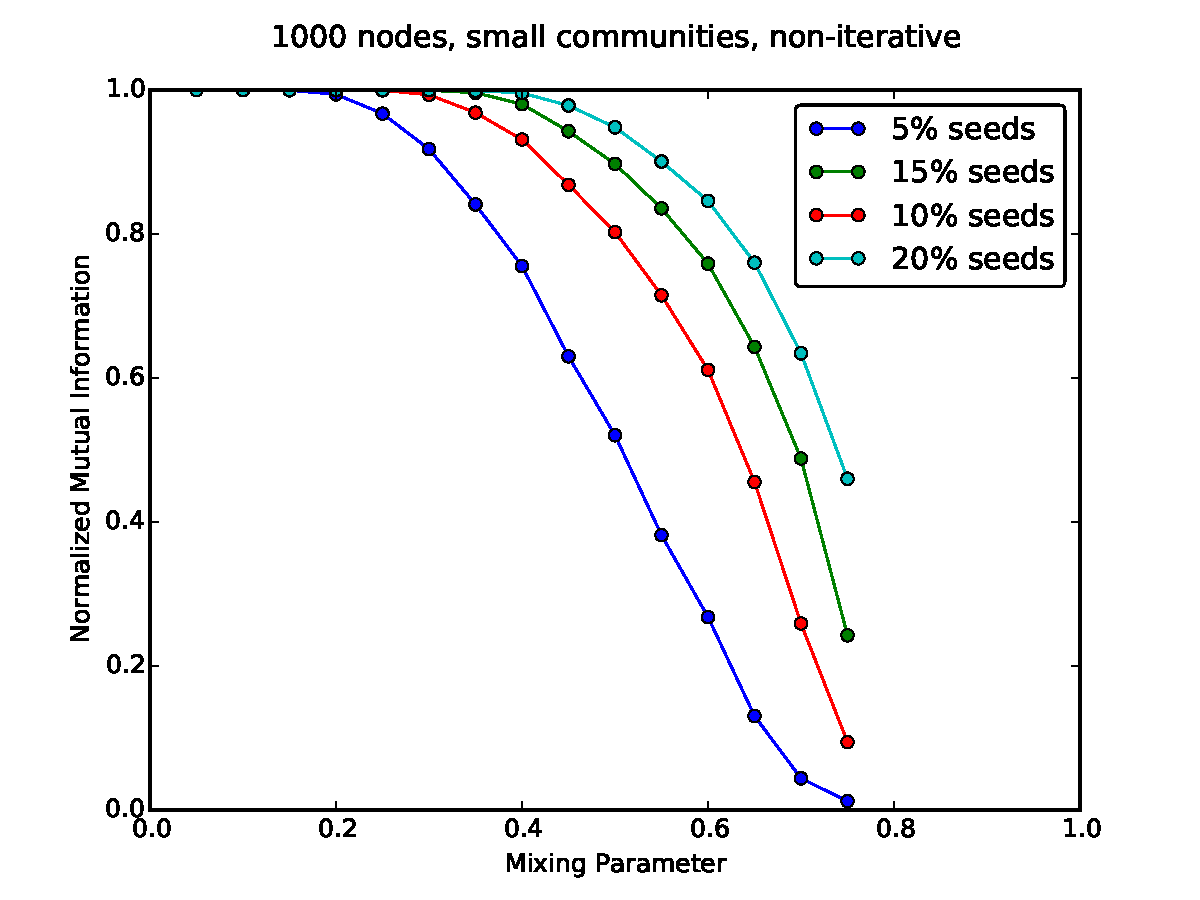
\includegraphics[width=\plotwidth]{plots/nonoverlap_noniter_a.pdf}
    \end{subfigure}%
    \begin{subfigure}{0.4\textwidth}
    \centering
    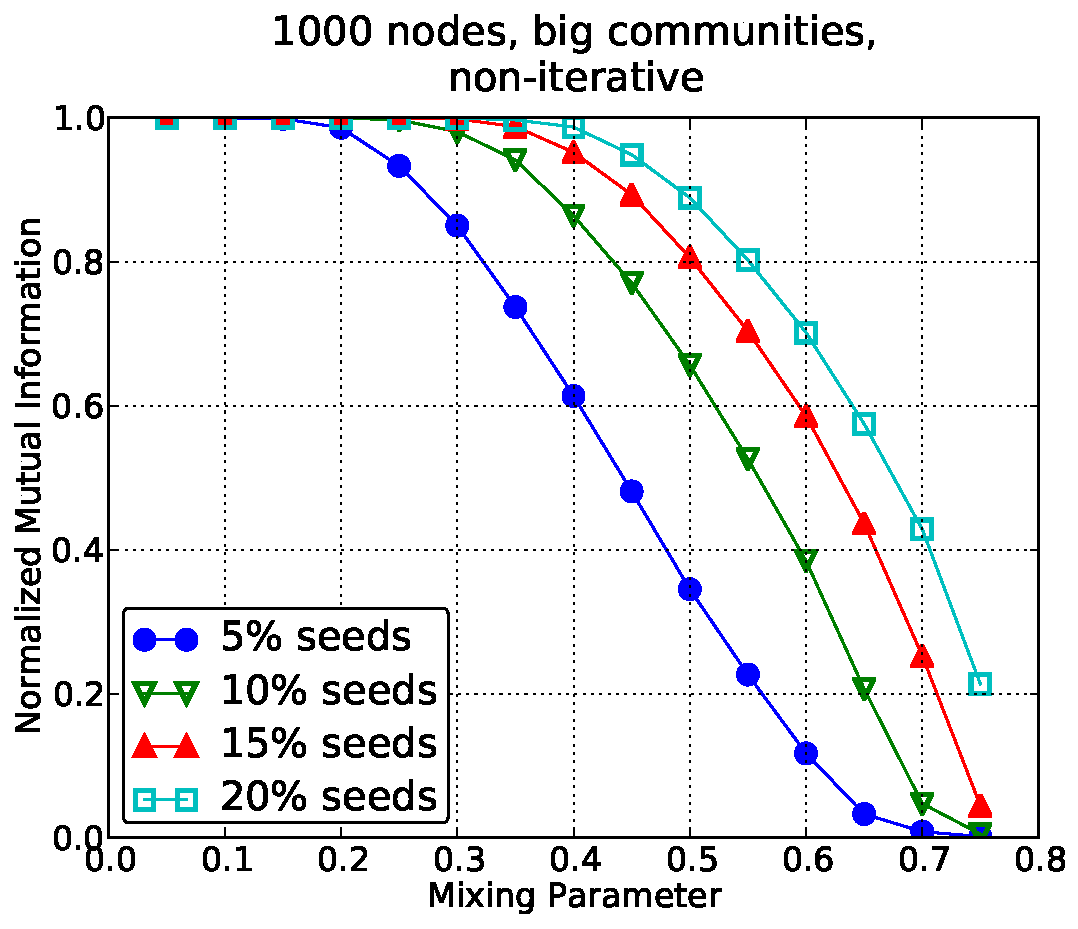
\includegraphics[width=\plotwidth]{plots/nonoverlap_noniter_b.pdf}
    \end{subfigure}
    \begin{subfigure}{0.4\textwidth}
    \centering
    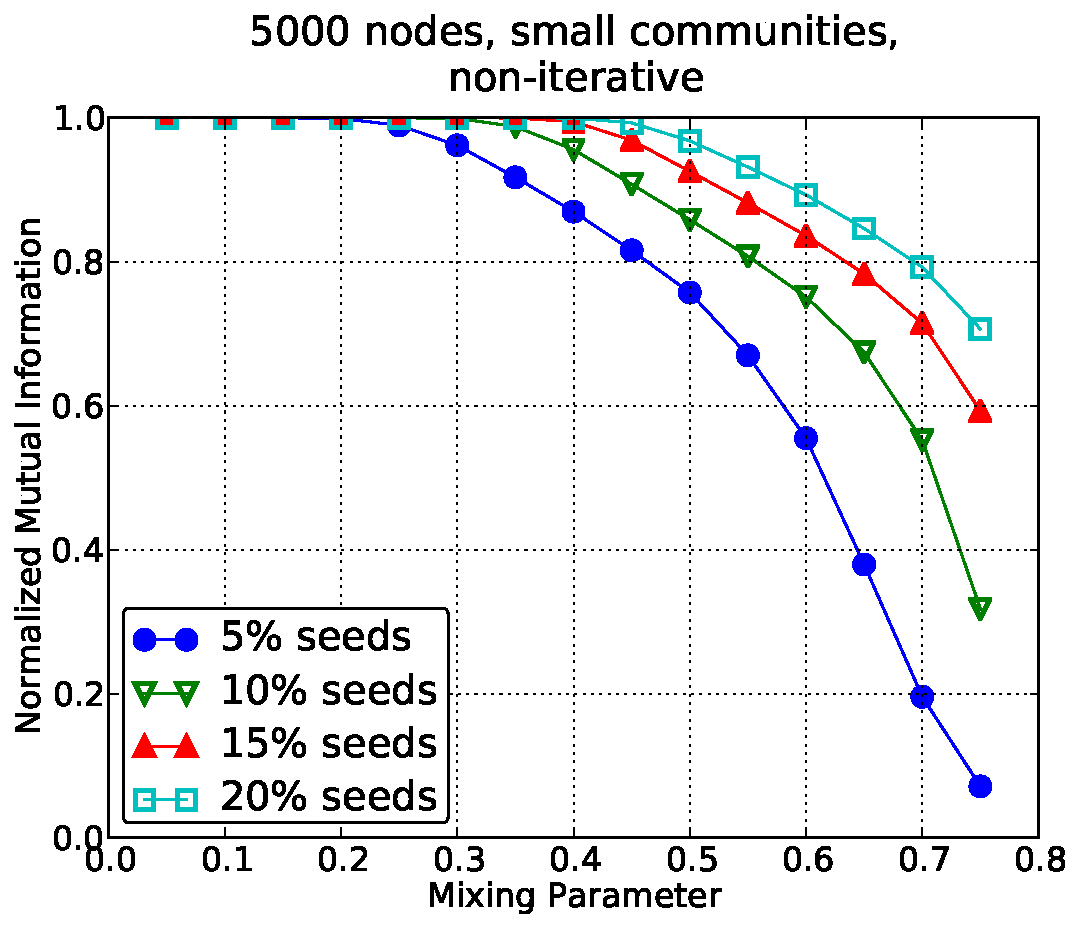
\includegraphics[width=\plotwidth]{plots/nonoverlap_noniter_c.pdf}
    \end{subfigure}%
    \begin{subfigure}{0.4\textwidth}
    \centering
    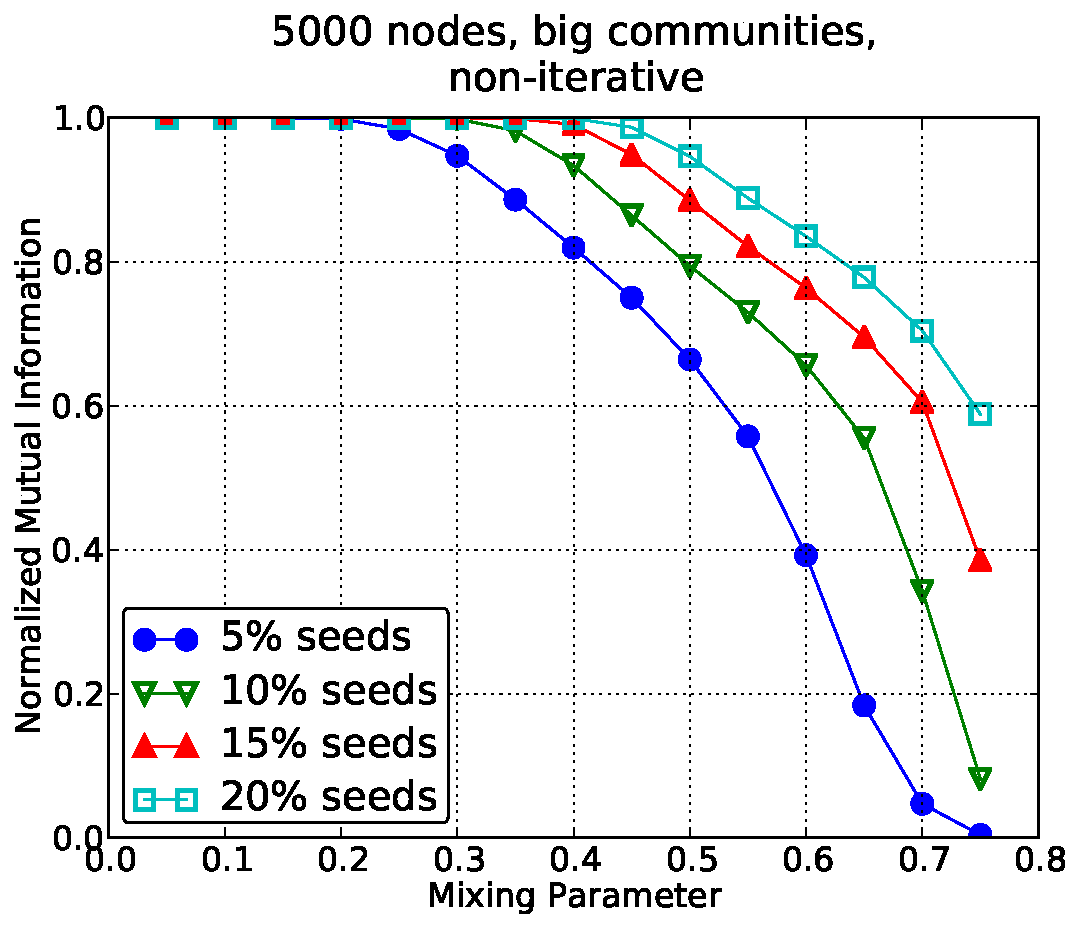
\includegraphics[width=\plotwidth]{plots/nonoverlap_noniter_d.pdf}
    \end{subfigure}
    \caption{Noniterative method for nonoverlapping communities.}\label{fig:no_iter_no_overlap}
\end{figure}
%
\begin{figure}[h!]
    \centering
    \begin{subfigure}{0.4\textwidth}
    \centering
    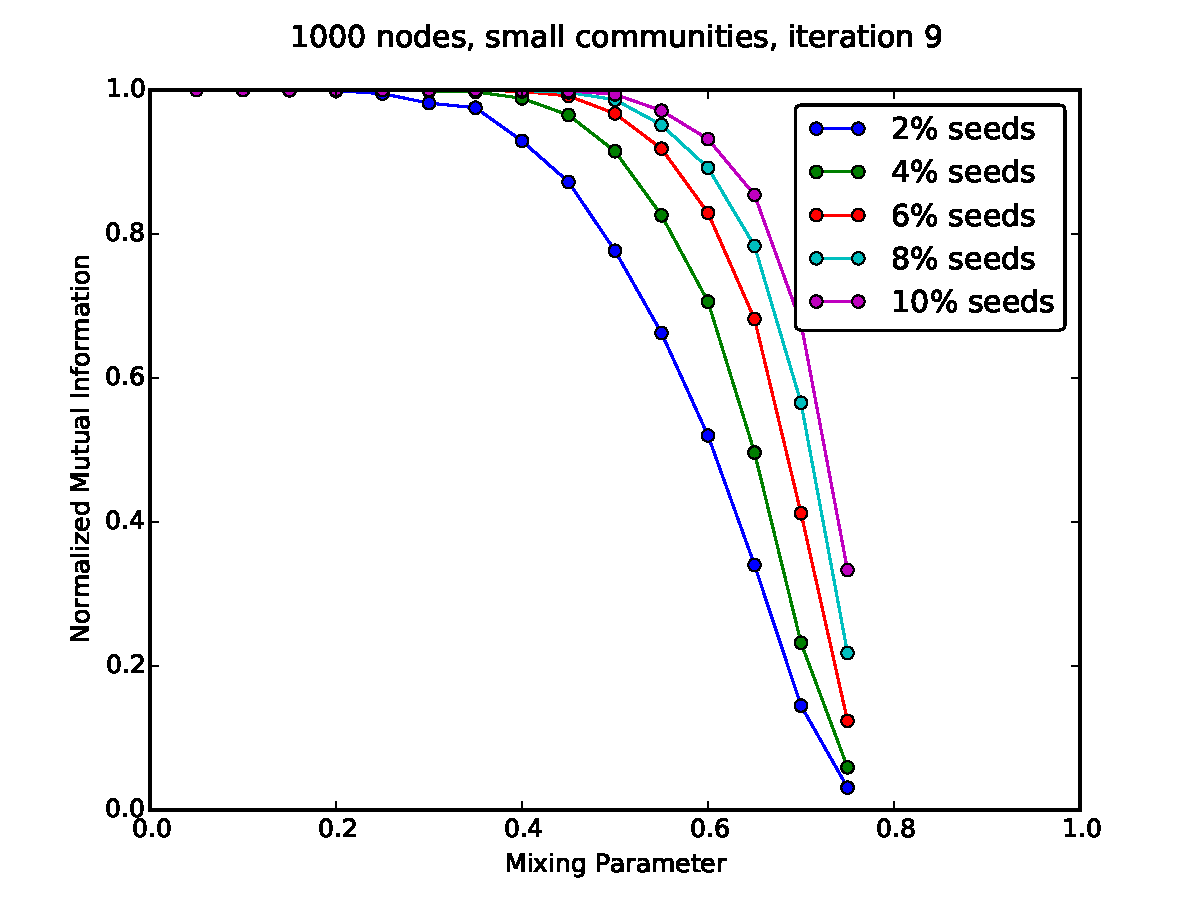
\includegraphics[width=\plotwidth]{plots/nonoverlap_iter_a.pdf}
    \end{subfigure}%
    \begin{subfigure}{0.4\textwidth}
    \centering
    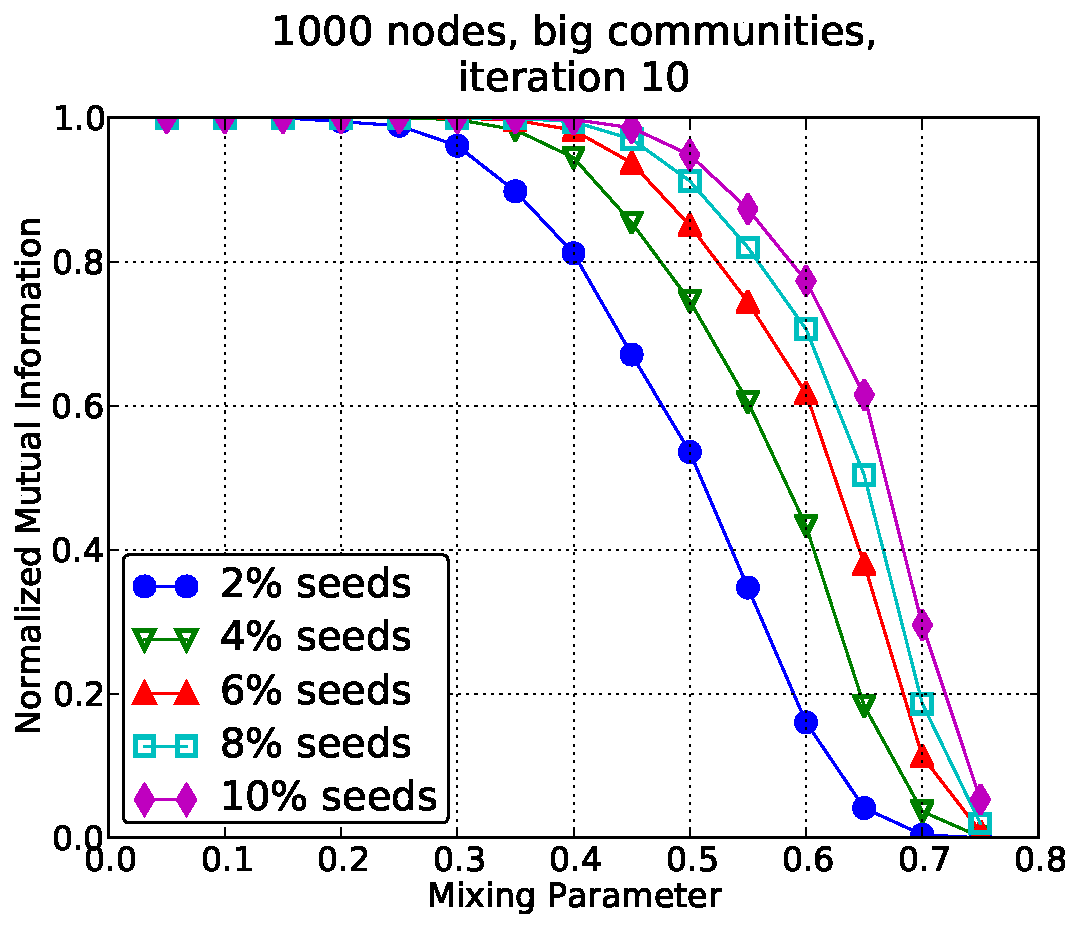
\includegraphics[width=\plotwidth]{plots/nonoverlap_iter_b.pdf}
    \end{subfigure}
    \begin{subfigure}{0.4\textwidth}
    \centering
    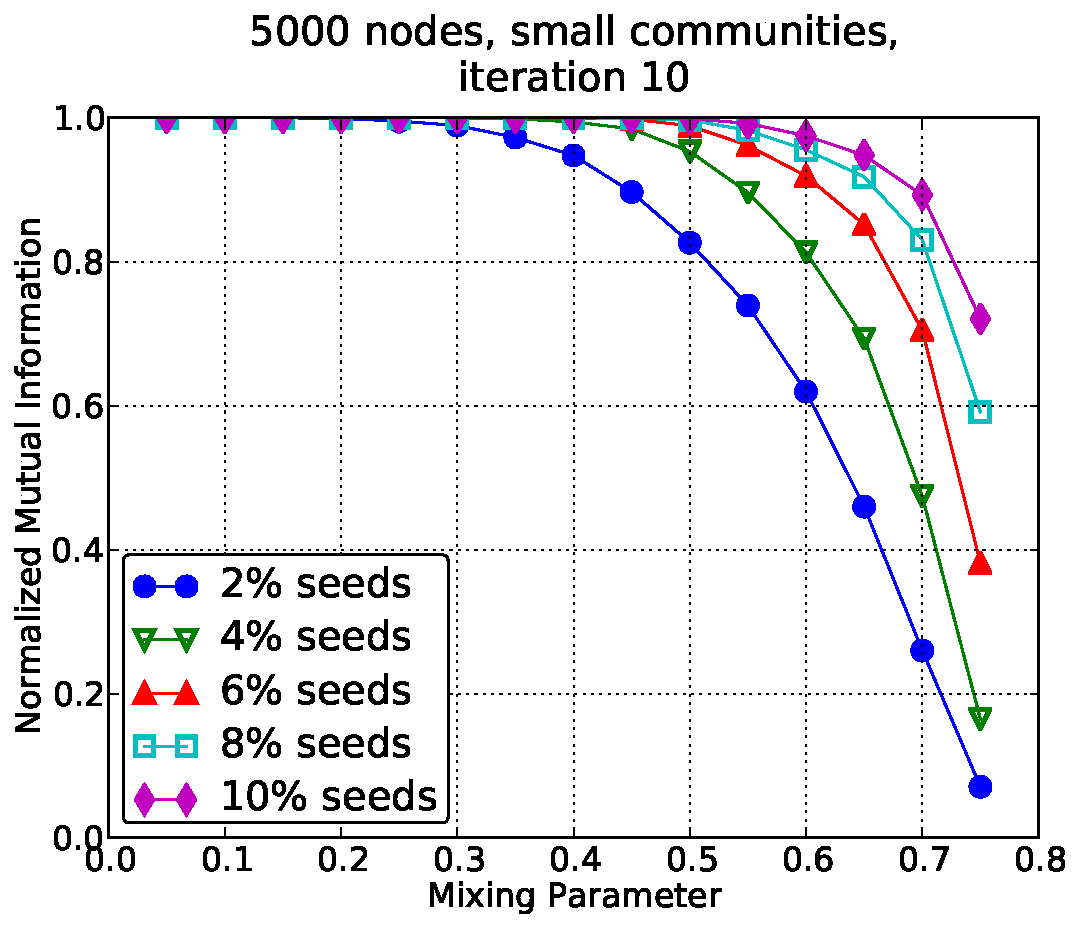
\includegraphics[width=\plotwidth]{plots/nonoverlap_iter_c.pdf}
    \end{subfigure}%
    \begin{subfigure}{0.4\textwidth}
    \centering
    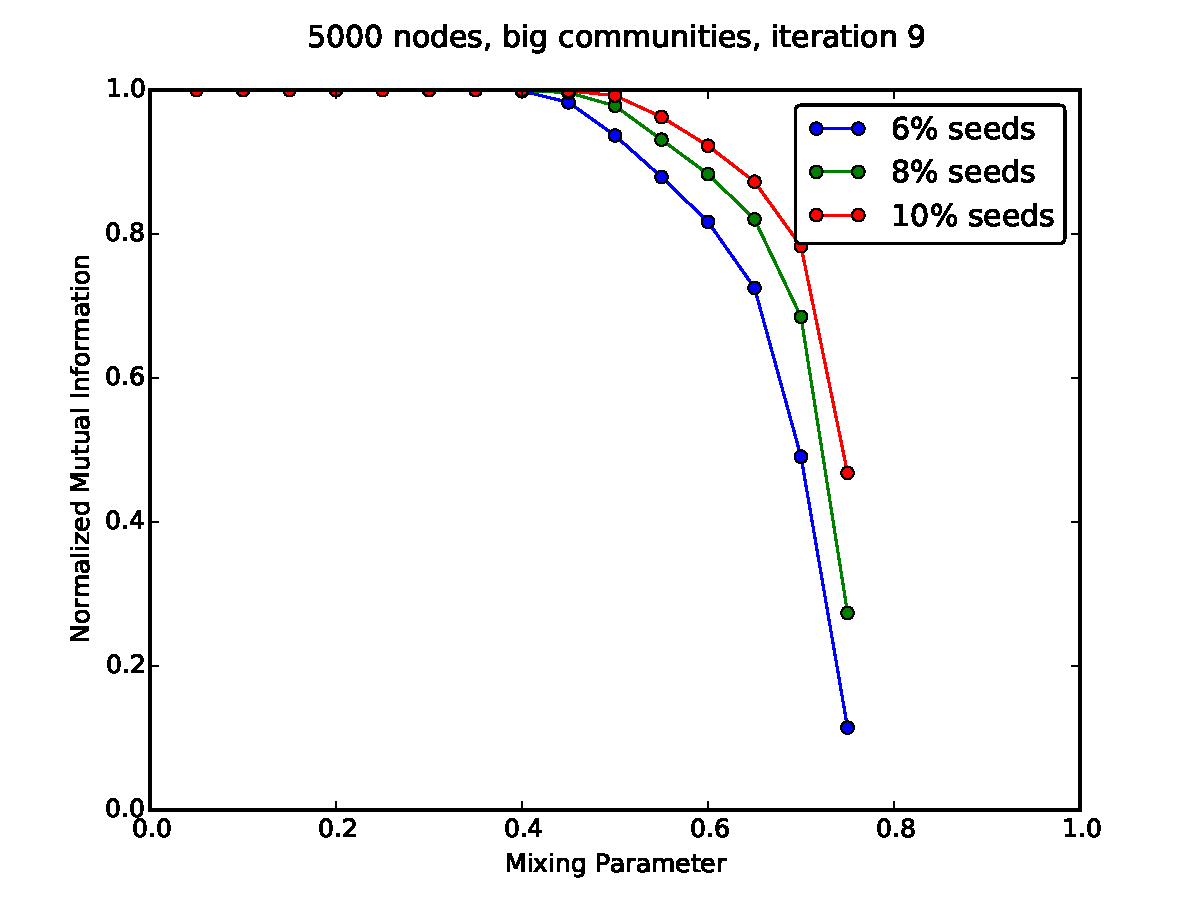
\includegraphics[width=\plotwidth]{plots/nonoverlap_iter_d.pdf}
    \end{subfigure}
    \caption{Iterative method for nonoverlapping communities.}\label{fig:iter_no_overlap}
\end{figure}
%
\begin{figure}[h]
    \centering
    \begin{subfigure}{0.4\textwidth}
    \centering
    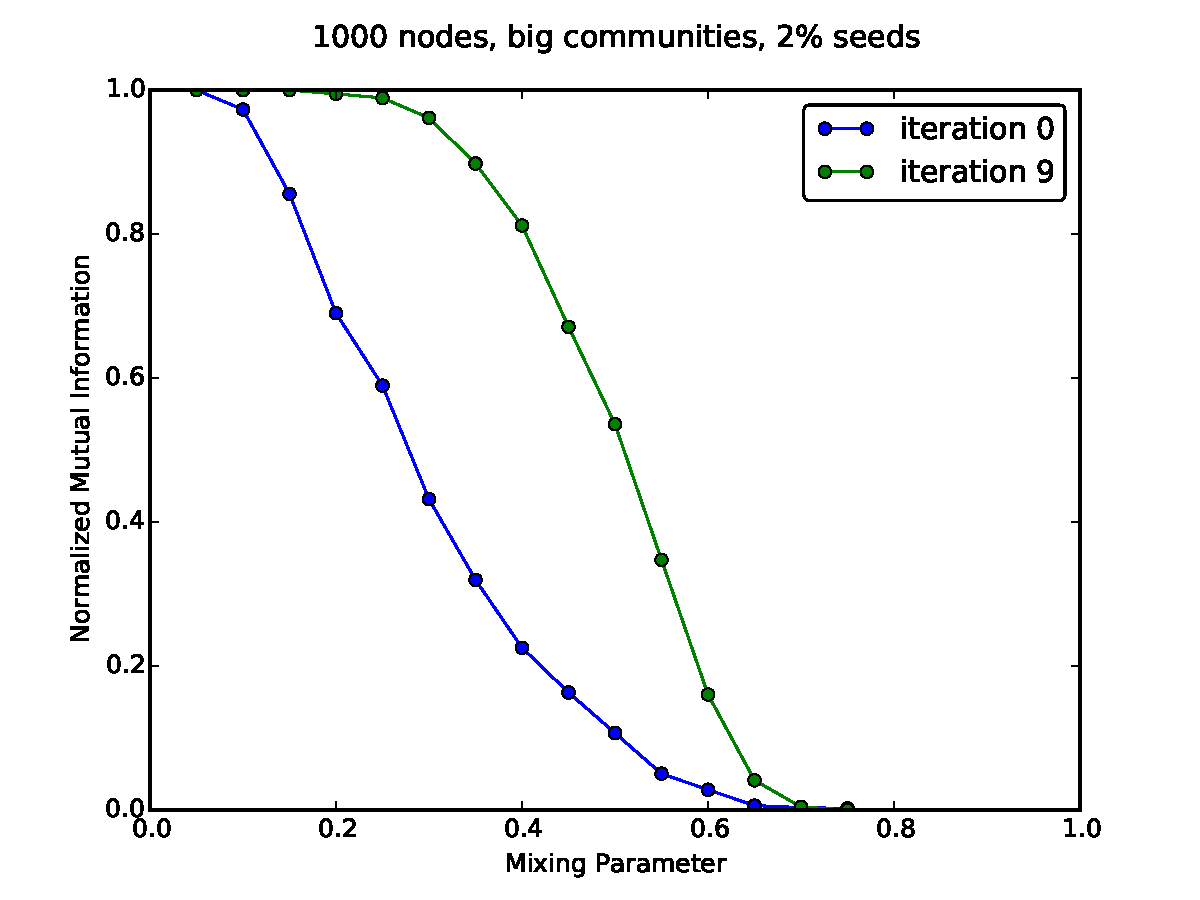
\includegraphics[width=\plotwidth]{plots/nonoverlap_compare_a.pdf}
    \end{subfigure}%
    \begin{subfigure}{0.4\textwidth}
    \centering
    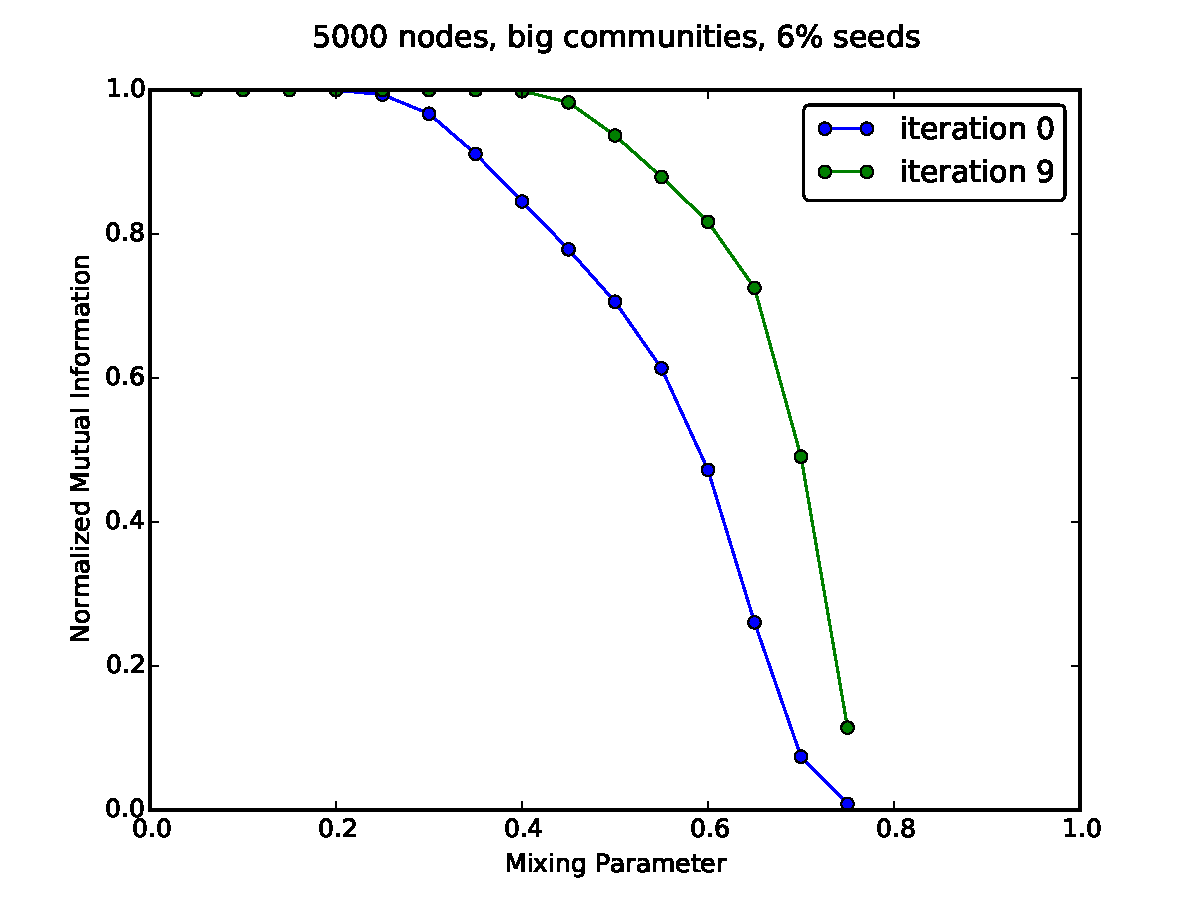
\includegraphics[width=\plotwidth]{plots/nonoverlap_compare_b.pdf}
    \end{subfigure}
    \caption{Comparison between the the iterative and non-iterative method for non-overlapping communities.}\label{fig:compare_iter_no_overlap}
\end{figure}
%
\begin{figure}[h!]
    \centering
    \begin{subfigure}{0.33\textwidth}
    \centering
    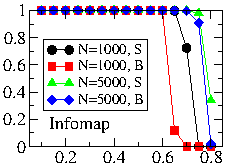
\includegraphics[width=\otherplotswidth]{lfrpaper/1_split_kropped.pdf}
    \end{subfigure}%
    \begin{subfigure}{0.33\textwidth}
    \centering
    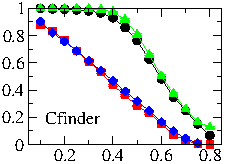
\includegraphics[width=\otherplotswidth]{lfrpaper/2_split_kropped.pdf}
    \end{subfigure}%
    \begin{subfigure}{0.33\textwidth}
    \centering
    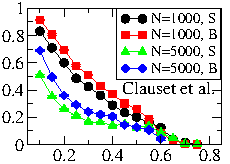
\includegraphics[width=\otherplotswidth]{lfrpaper/3_split_kropped.pdf}
    \end{subfigure}
    \begin{subfigure}{0.33\textwidth}
    \centering
    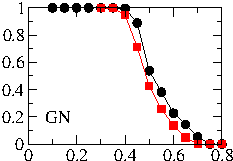
\includegraphics[width=\otherplotswidth]{lfrpaper/4_split_kropped.pdf}
    \end{subfigure}%
    \begin{subfigure}{0.33\textwidth}
    \centering
    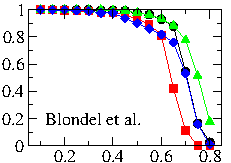
\includegraphics[width=\otherplotswidth]{lfrpaper/5_split_kropped.pdf}
    \end{subfigure}%
    \begin{subfigure}{0.33\textwidth}
    \centering
    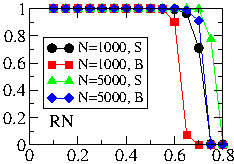
\includegraphics[width=\otherplotswidth]{lfrpaper/6_split_kropped.pdf}
    \end{subfigure}%
    \caption{
        Plots for Infomap, CFinder, the algorithm of Clauset \etal, Girvan-Newman (GN), Blondel \etal, 
        and the Pott's model approach by Ronhovde and Nussinov (RN) on the LFR benchmark for non-overlapping 
		communities. As usual, the NMI-value ($y$-axis) is plotted against the mixing factor ($x$-axis).
        Tests were performed on graphs with 1000 and 5000 nodes with big (B) and small (S) communities.
        These figures are taken from~\cite{LF09}.
    }
\end{figure}



\subsection{Overlapping communities}
Figures~\ref{fig:no_iter_overlap_1000N} and~\ref{fig:no_iter_overlap_5000N} 
show our results for the overlapping case. In the study of Lancichinetti and Fortunato~\cite{LF09}, 
only one algorithm (\emph{Cfinder}~\cite{PDFV05}) for overlapping communities was benchmarked. 
The main difference with the non-overlapping case is that typically our algorithm needs a larger 
seed node percentage per community. This is not surprising since in the overlapping case, we would 
need seed nodes from the various overlaps as well as from the non-overlapping portions of communities 
to make a good-enough calculation of the affinities. 

For graphs of both 1000 and 5000 nodes, our algorithm performs better 
than Cfinder upto an overlapping fraction of $0.4$. We stress that Cfinder 
has an exponential worst-case running time and would be infeasible on larger graphs. 
%
%The best case scenario for Cfinder The important fact is that our algorithm performs 
%a lot better on LFR benchmark graphs for 
%a mixing factor of $0.3$. In the most extreme case of $1000$ nodes, big communities 
%and a mixing factor of $0.3$ the \textit{CFinder} algorithm has $60$ percent NMI as 
%its best result at zero percent overlapping nodes, and goes only down if one increases 
%the fraction of overlapping nodes, whereas our algorithm starts at $80$ percent NMI 
%even for $5$ percent seed nodes. If we use at least $10$ percent we can go up to 
%an overlap of $0.3$ before we reach $60$ percent NMI.
%
%For $5000$ nodes the results are similar but not as extreme. In conclusion we can 
%say that our algorithm seems to perform better on LFR graphs and offers a better runtime 
%compared to that of the exponential worst-case runtime of \textit{CFinder}.

Figures~\ref{fig:iter_overlap_1000N} and~\ref{fig:iter_overlap_5000N} show the 
plots for the iterative method. A comparison of the non-iteratve and iterative method 
is shown in Figure~\ref{fig:compare_iter_overlap}. Iteration yields an improvement in performance,
as measured by the NMI, but it is not as dramatic as in the non-overlapping case 
with the NMI increase being at most $10\%$ at best. The percentage of seed nodes per community required in the iterative 
approach with a mixing factor of $0.3$ is around 8$\%$. 


\begin{figure}[h!]
    \centering
    \begin{subfigure}{0.4\textwidth}
    \centering
    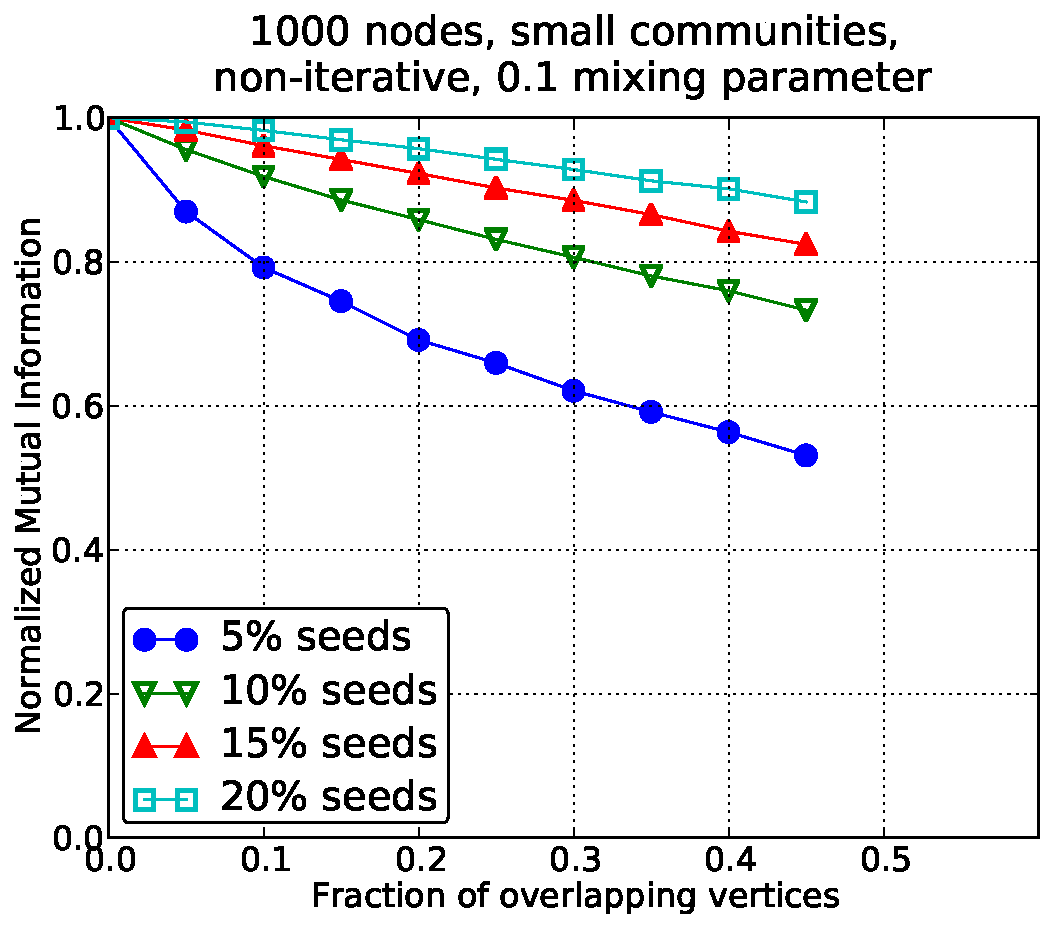
\includegraphics[width=\plotwidth]{plots/overlap_noniter_1mu_a.pdf}
    \end{subfigure}%
    \begin{subfigure}{0.4\textwidth}
    \centering
    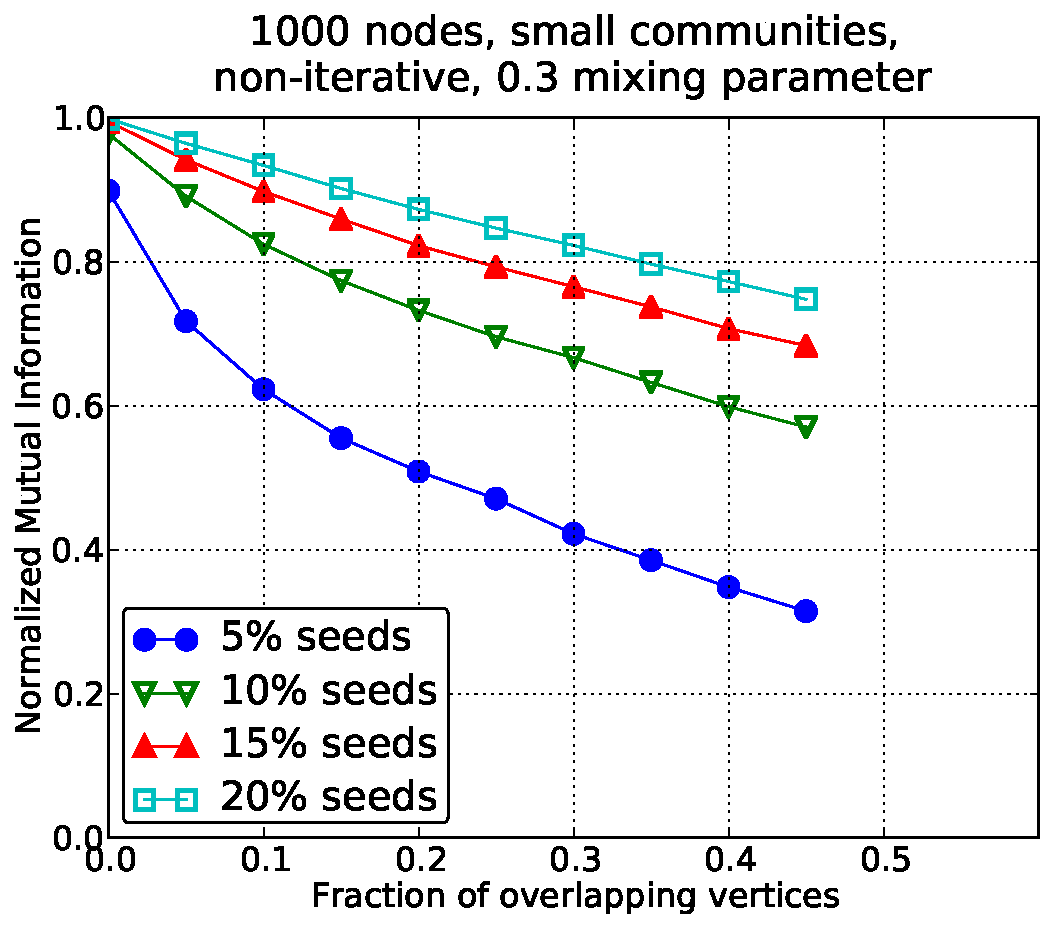
\includegraphics[width=\plotwidth]{plots/overlap_noniter_3mu_a.pdf}
    \end{subfigure}
    \begin{subfigure}{0.4\textwidth}
    \centering
    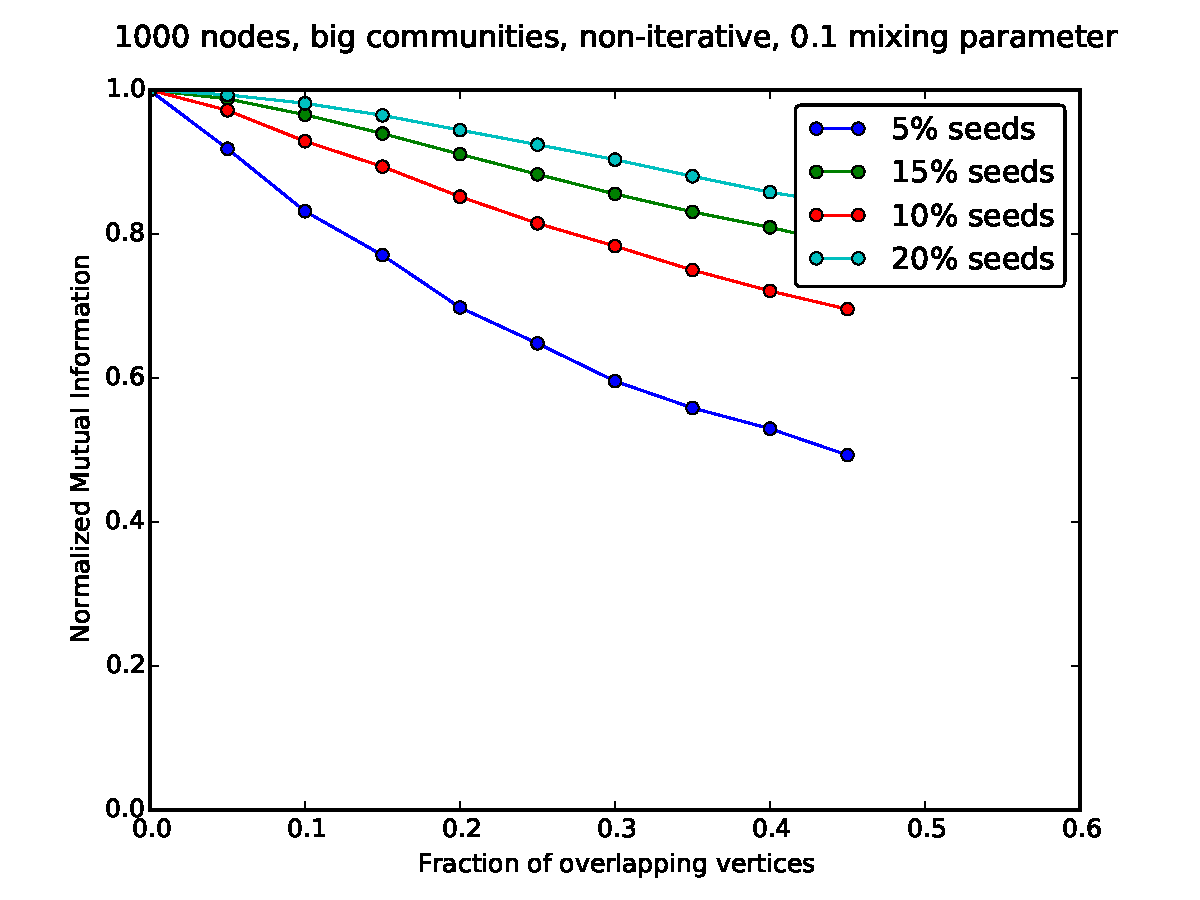
\includegraphics[width=\plotwidth]{plots/overlap_noniter_1mu_b.pdf}
    \end{subfigure}%
    \begin{subfigure}{0.4\textwidth}
    \centering
    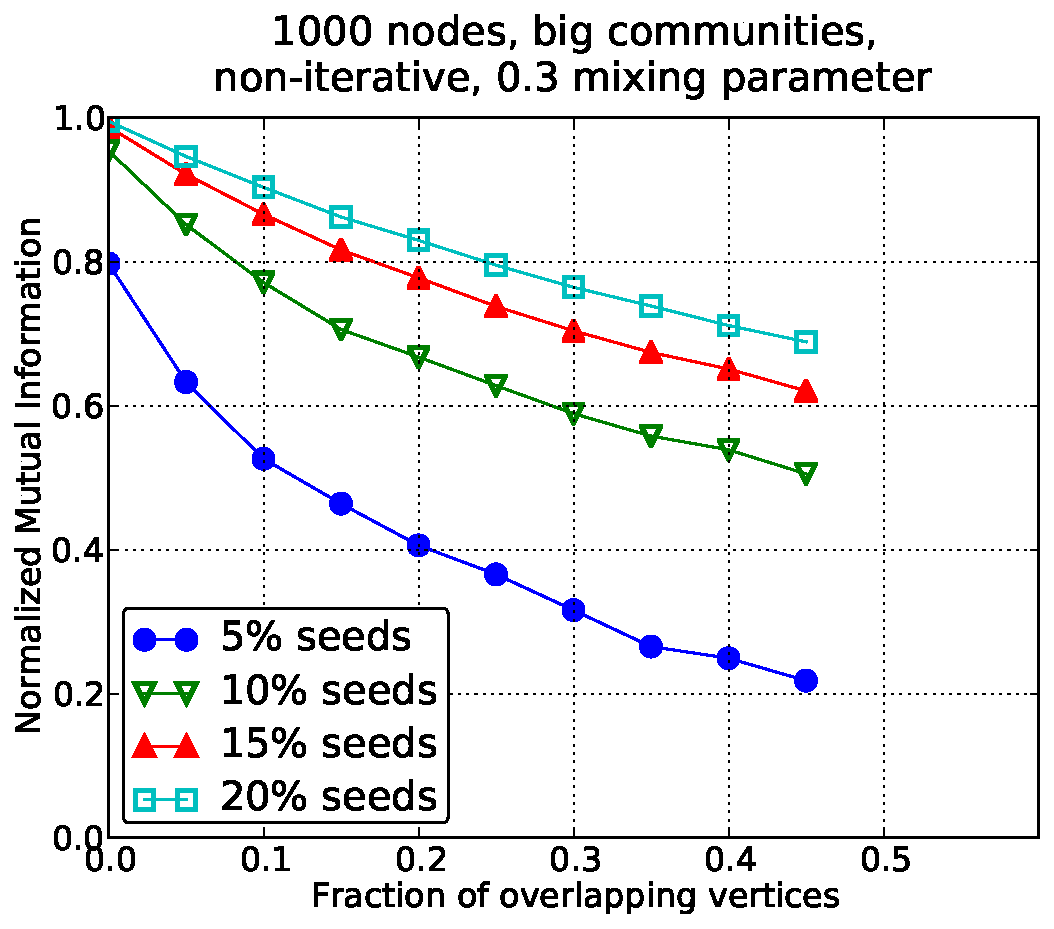
\includegraphics[width=\plotwidth]{plots/overlap_noniter_3mu_b.pdf}
    \end{subfigure}
    \caption{Noniterative method for overlapping communities on 1000 nodes.}\label{fig:no_iter_overlap_1000N}
\end{figure}
%
\begin{figure}[h!]
    \centering
    \begin{subfigure}{0.4\textwidth}
    \centering
    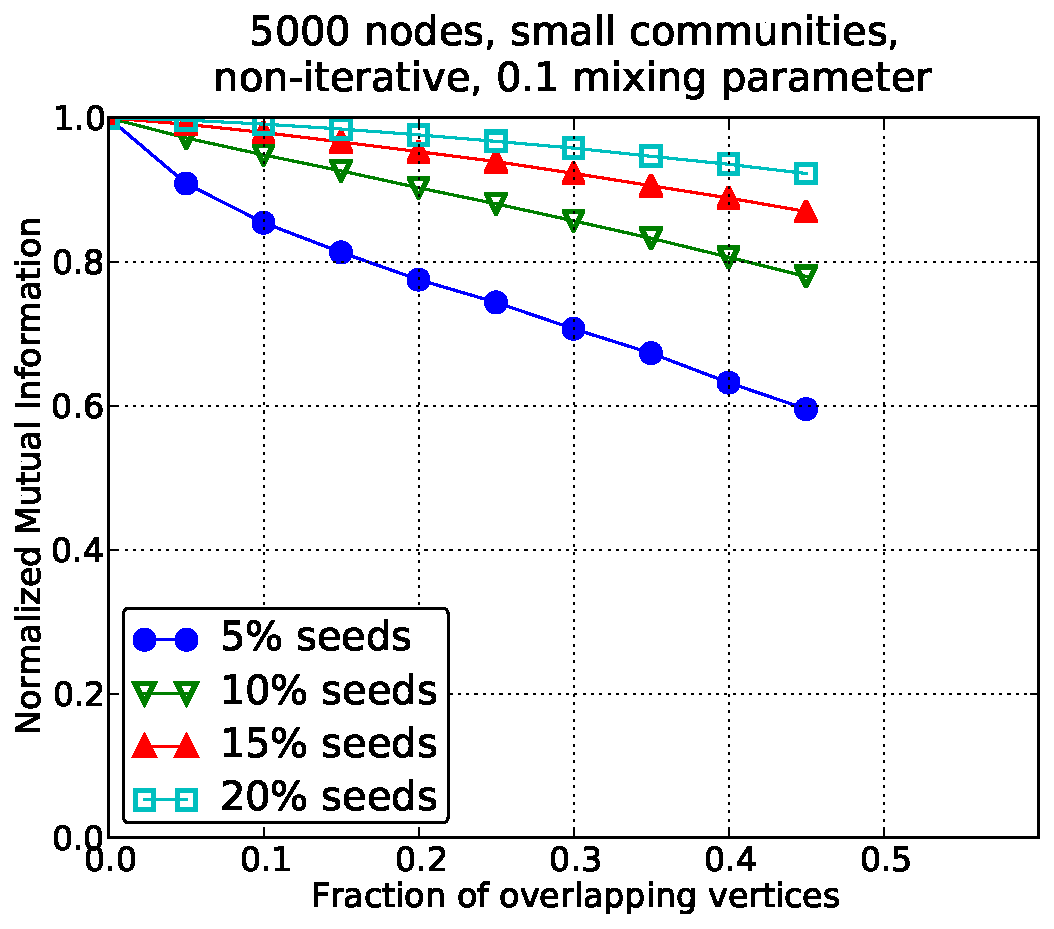
\includegraphics[width=\plotwidth]{plots/overlap_noniter_1mu_c.pdf}
    \end{subfigure}%
    \begin{subfigure}{0.4\textwidth}
    \centering
    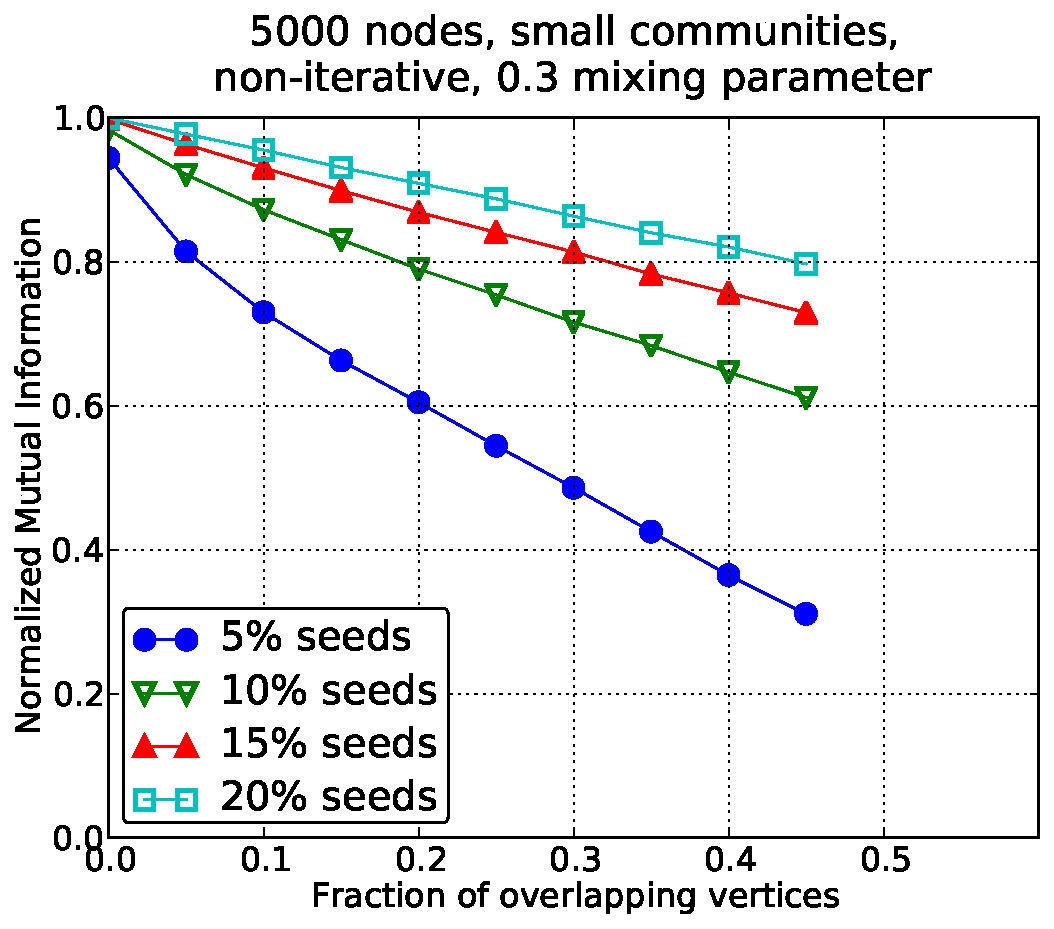
\includegraphics[width=\plotwidth]{plots/overlap_noniter_3mu_c.pdf}
    \end{subfigure}
    \begin{subfigure}{0.4\textwidth}
    \centering
    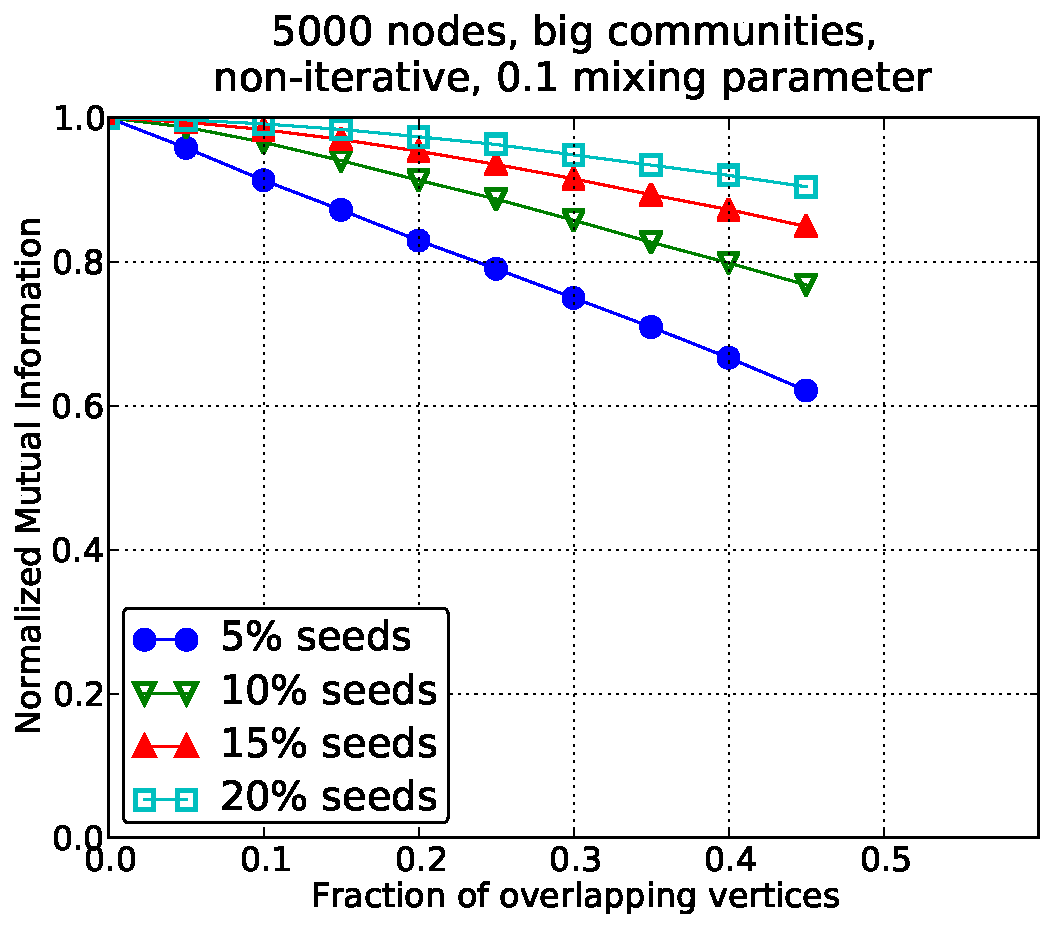
\includegraphics[width=\plotwidth]{plots/overlap_noniter_1mu_d.pdf}
    \end{subfigure}%
    \begin{subfigure}{0.4\textwidth}
    \centering
    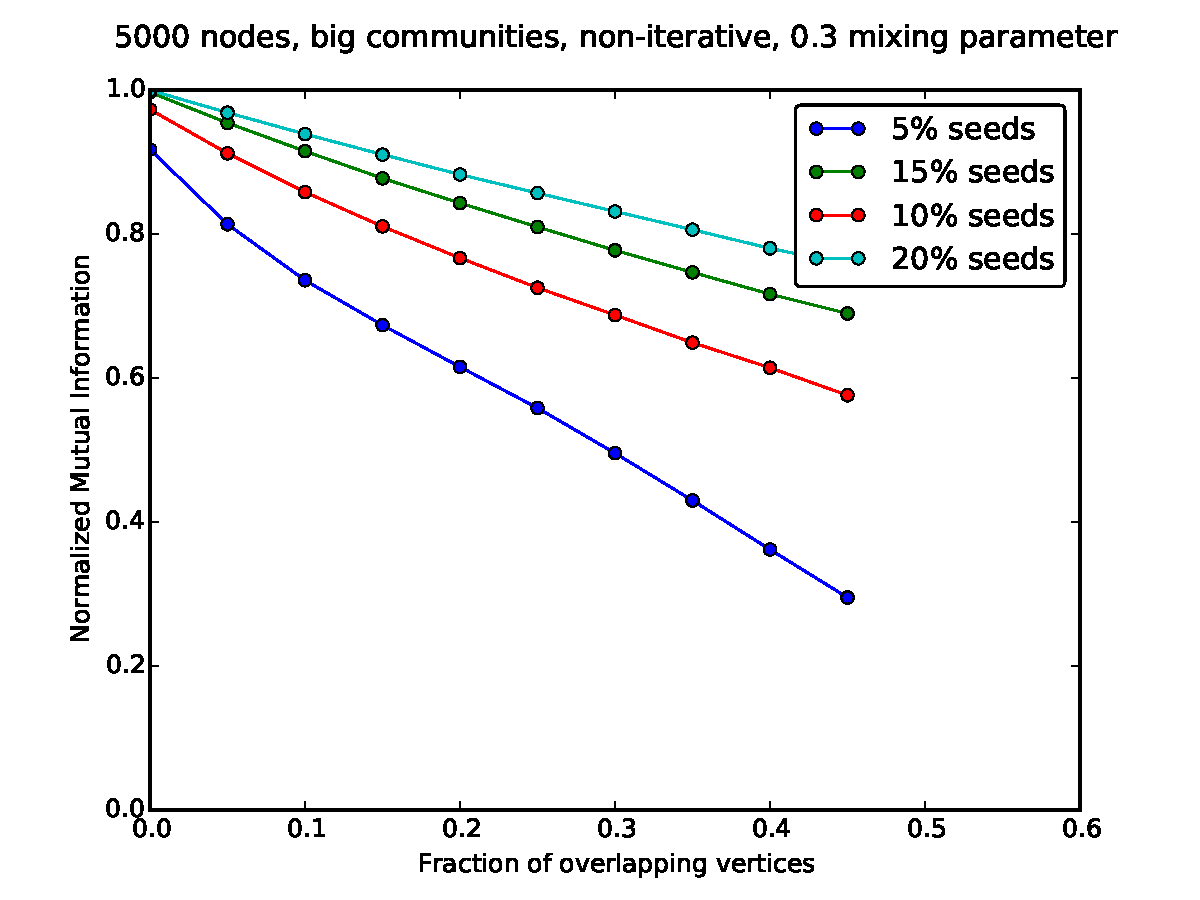
\includegraphics[width=\plotwidth]{plots/overlap_noniter_3mu_d.pdf}
    \end{subfigure}
    \caption{Noniterative method for overlapping communities on 5000 nodes.}\label{fig:no_iter_overlap_5000N}
\end{figure}
%
\begin{figure}[h!]
    \centering
    \begin{subfigure}{0.4\textwidth}
    \centering
    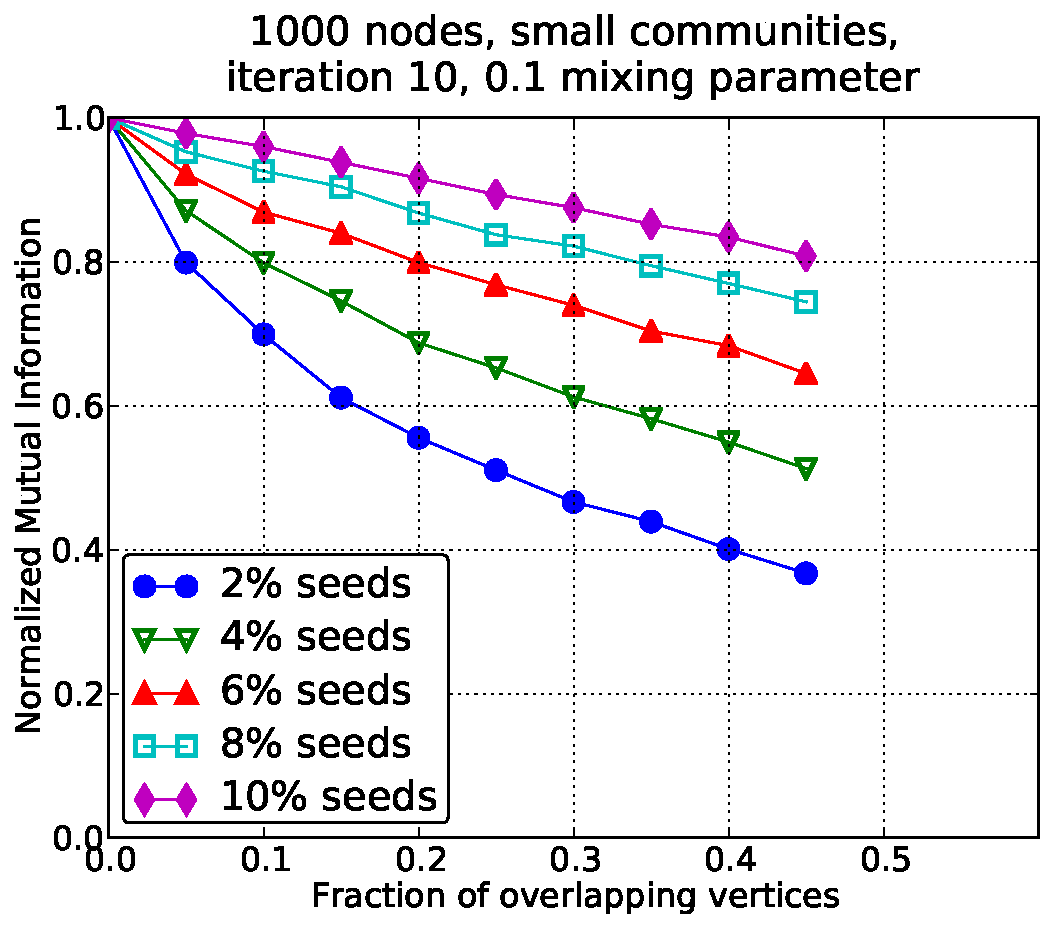
\includegraphics[width=\plotwidth]{plots/overlap_iter_1mu_a.pdf}
    \end{subfigure}%
    \begin{subfigure}{0.4\textwidth}
    \centering
    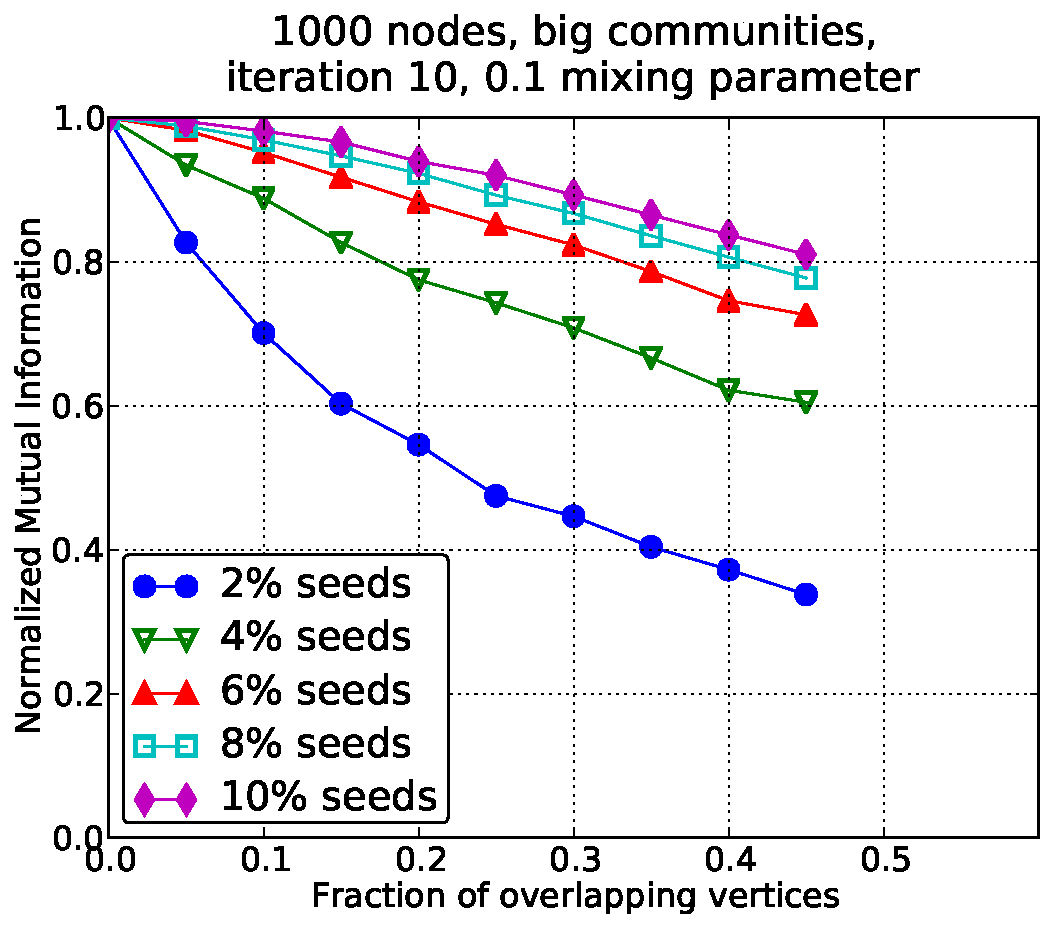
\includegraphics[width=\plotwidth]{plots/overlap_iter_1mu_b.pdf}
    \end{subfigure}
    \begin{subfigure}{0.4\textwidth}
    \centering
    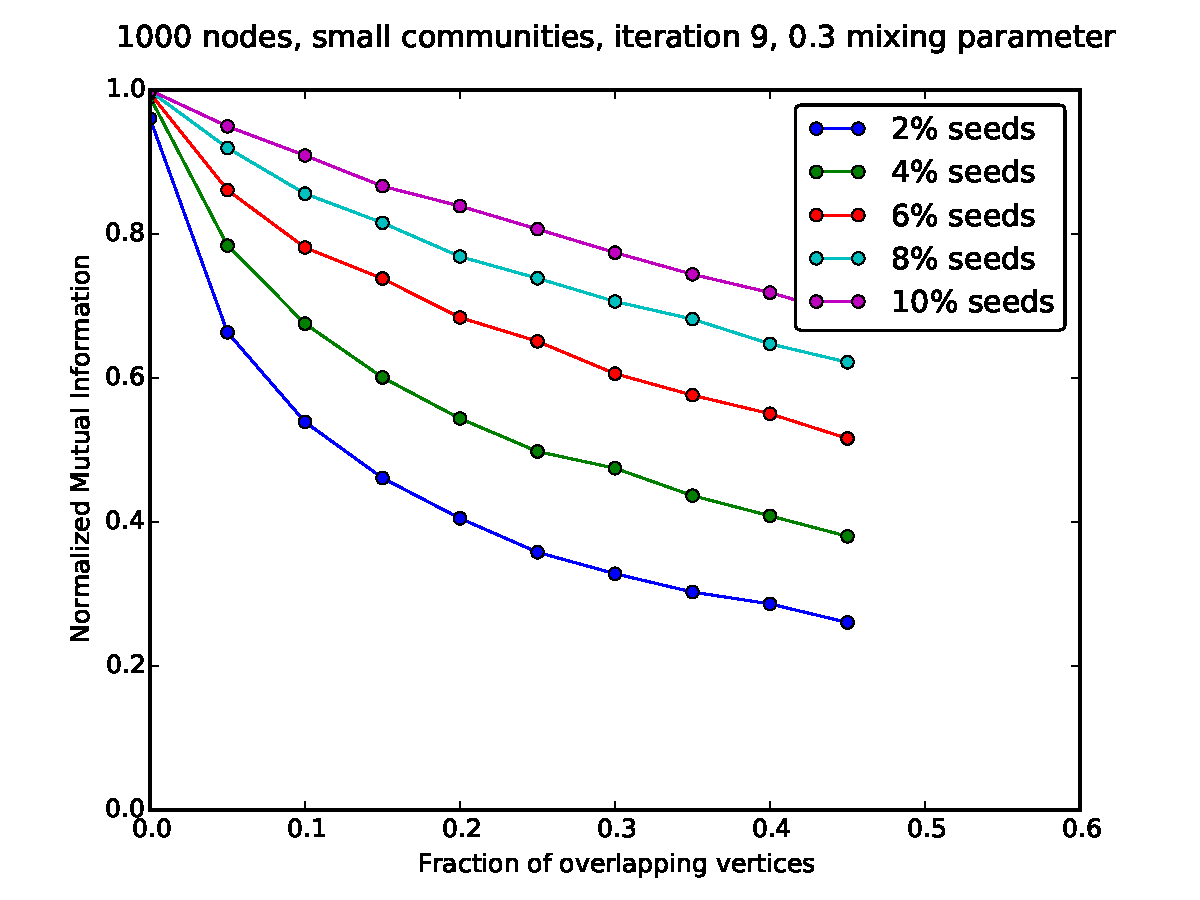
\includegraphics[width=\plotwidth]{plots/overlap_iter_3mu_a.pdf}
    \end{subfigure}%
    \begin{subfigure}{0.4\textwidth}
    \centering
    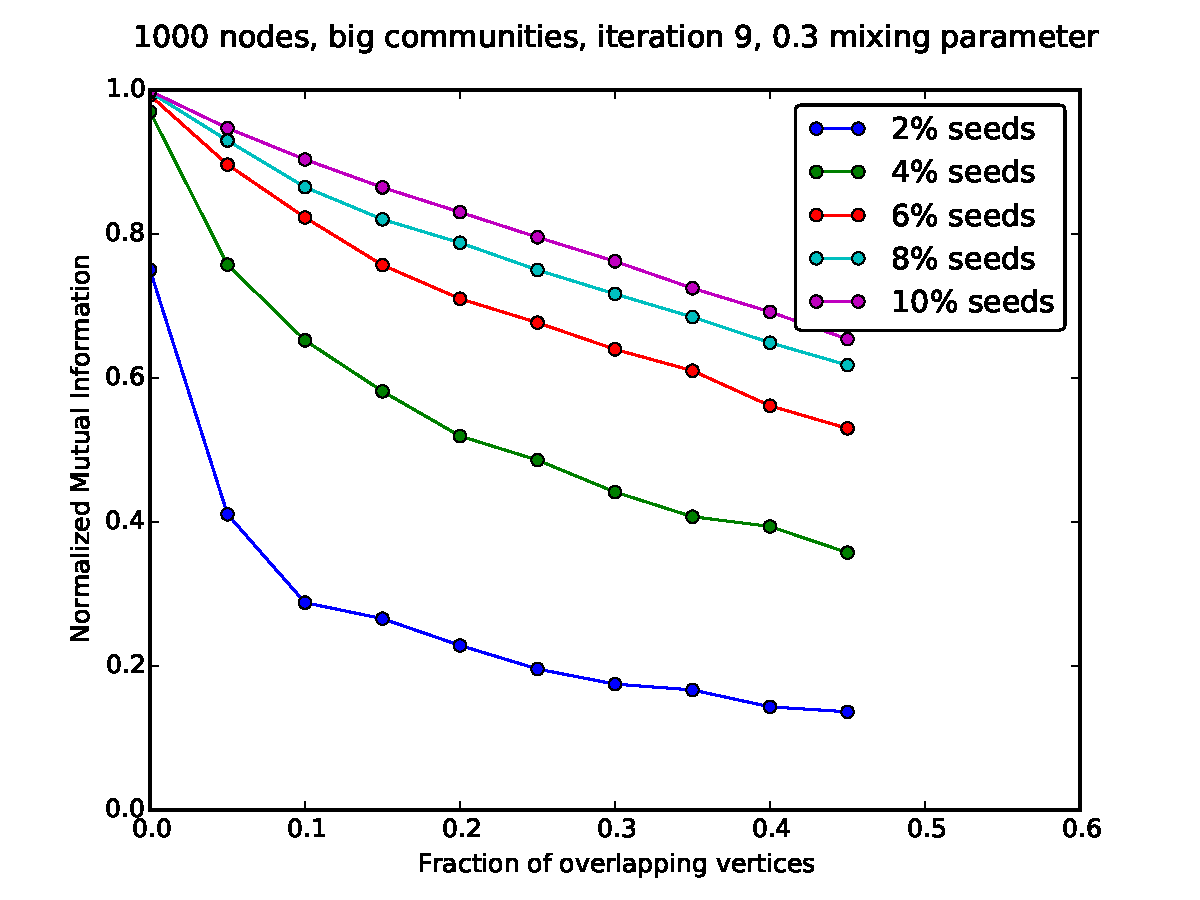
\includegraphics[width=\plotwidth]{plots/overlap_iter_3mu_b.pdf}
    \end{subfigure}
    \caption{Iterative method for overlapping communities on 1000 nodes.}\label{fig:iter_overlap_1000N}
\end{figure}
%
\begin{figure}[h!]
    \centering
    \begin{subfigure}{0.4\textwidth}
    \centering
    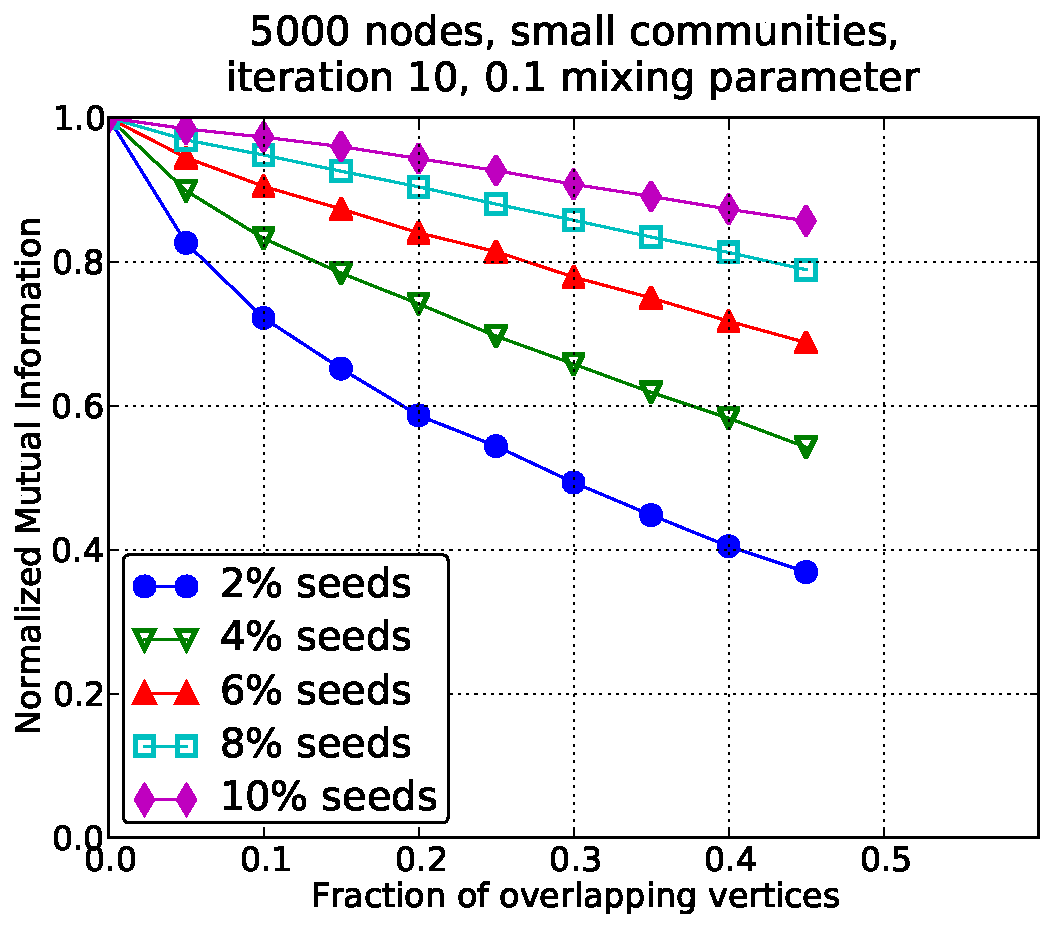
\includegraphics[width=\plotwidth]{plots/overlap_iter_1mu_c.pdf}
    \end{subfigure}%
    \begin{subfigure}{0.4\textwidth}
    \centering
    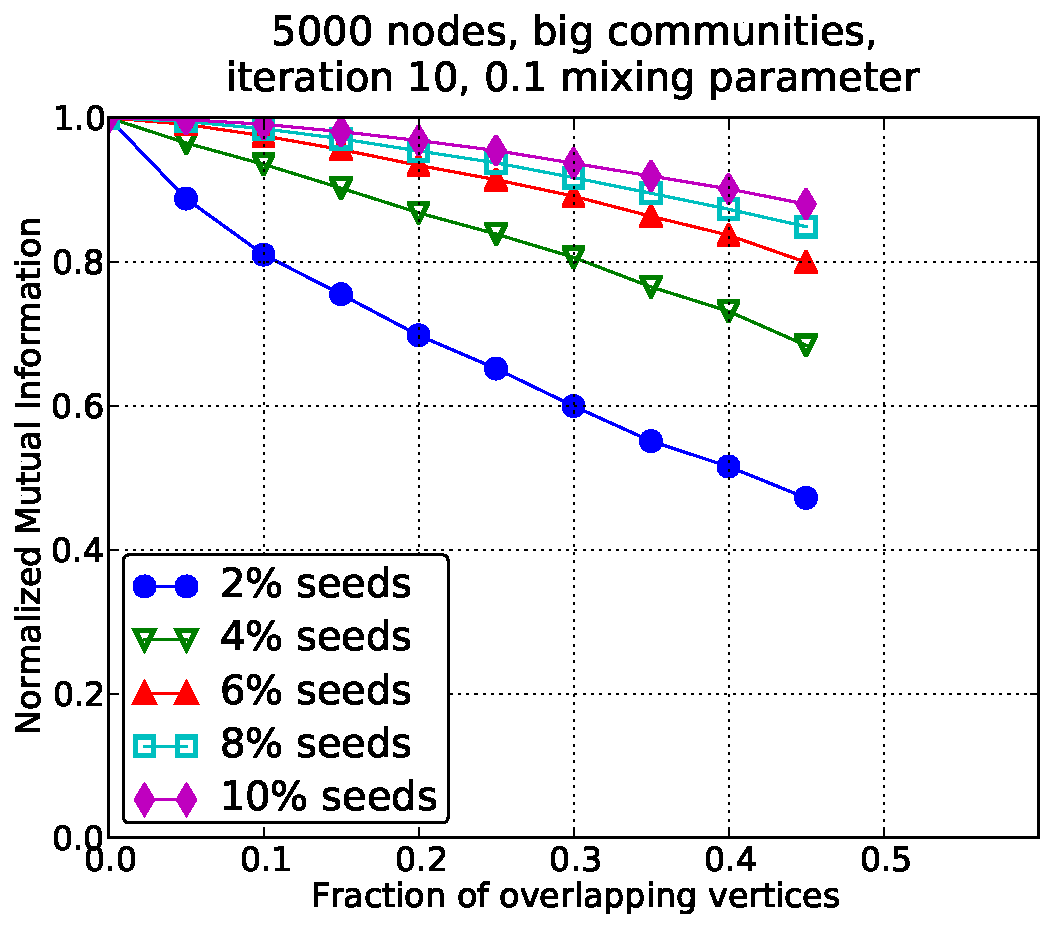
\includegraphics[width=\plotwidth]{plots/overlap_iter_1mu_d.pdf}
    \end{subfigure}
    \begin{subfigure}{0.4\textwidth}
    \centering
    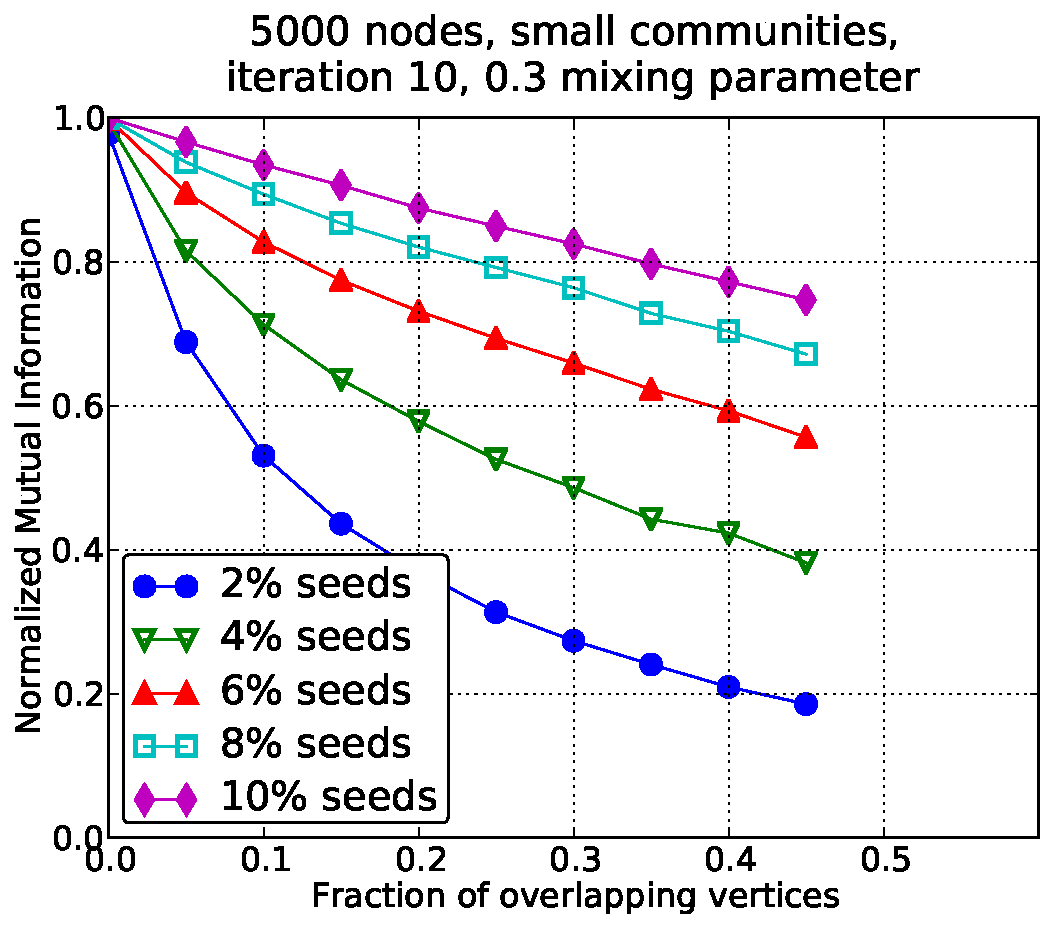
\includegraphics[width=\plotwidth]{plots/overlap_iter_3mu_c.pdf}
    \end{subfigure}%
    \begin{subfigure}{0.4\textwidth}
    \centering
    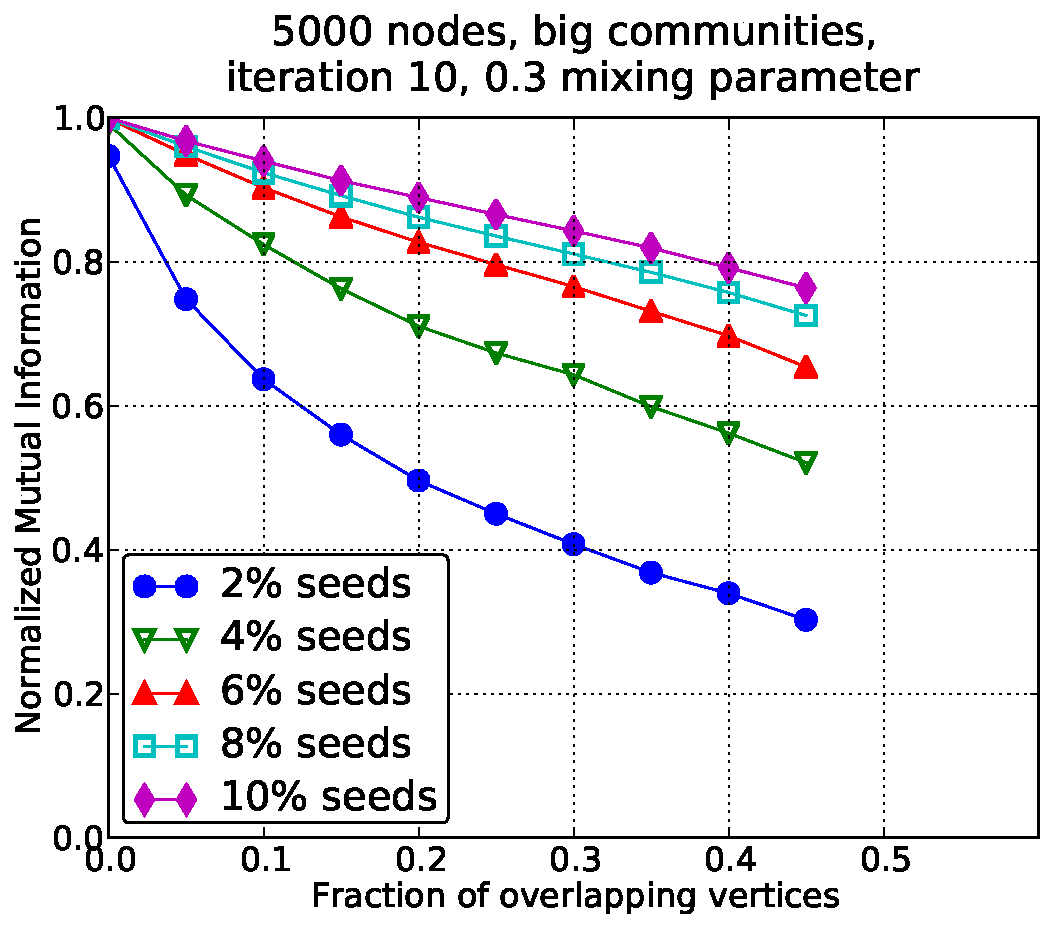
\includegraphics[width=\plotwidth]{plots/overlap_iter_3mu_d.pdf}
    \end{subfigure}
    \caption{Iterative method for overlapping communities on 5000 nodes.}\label{fig:iter_overlap_5000N}
\end{figure}
%
\begin{figure}[h!]
    \centering
    \begin{subfigure}{0.4\textwidth}
    \centering
    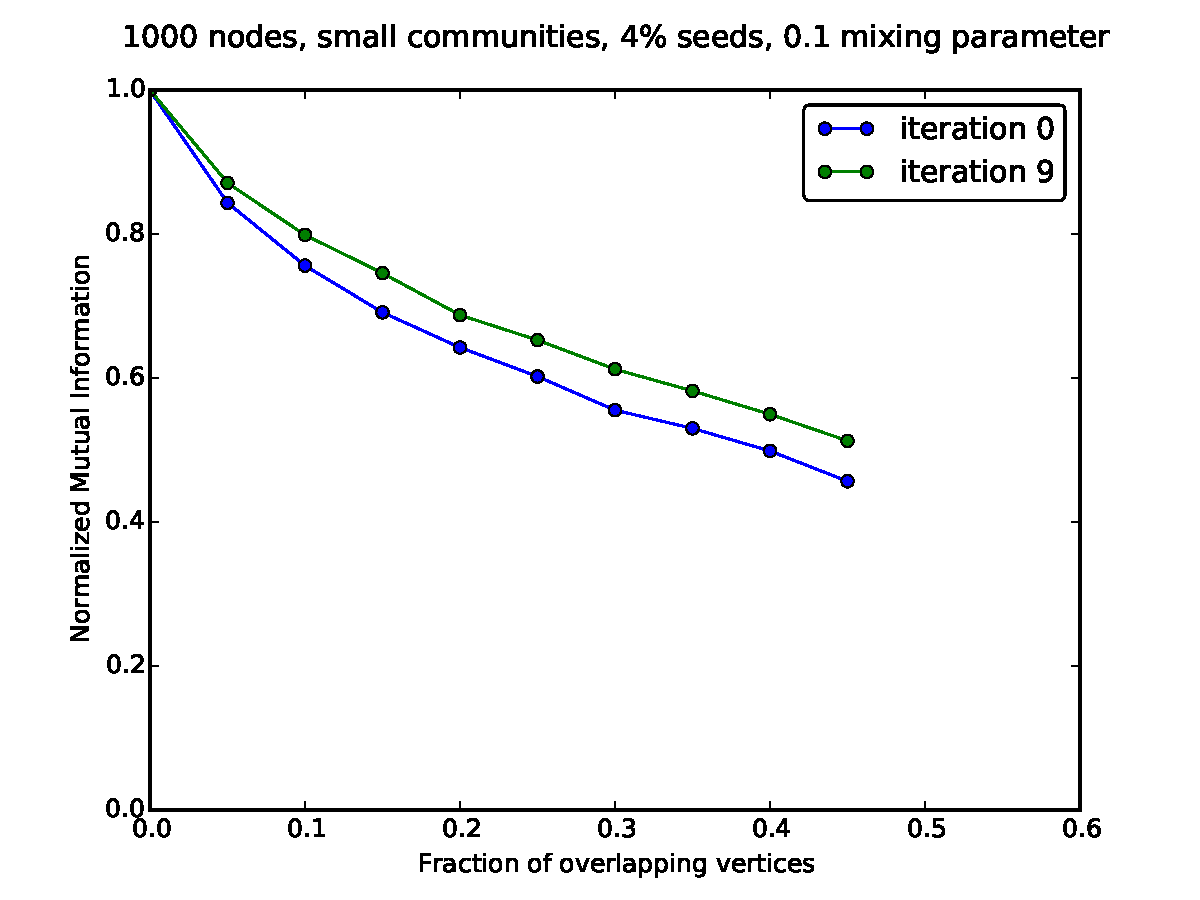
\includegraphics[width=\plotwidth]{plots/overlap_compare_a.pdf}
    \end{subfigure}%
    \begin{subfigure}{0.4\textwidth}
    \centering
    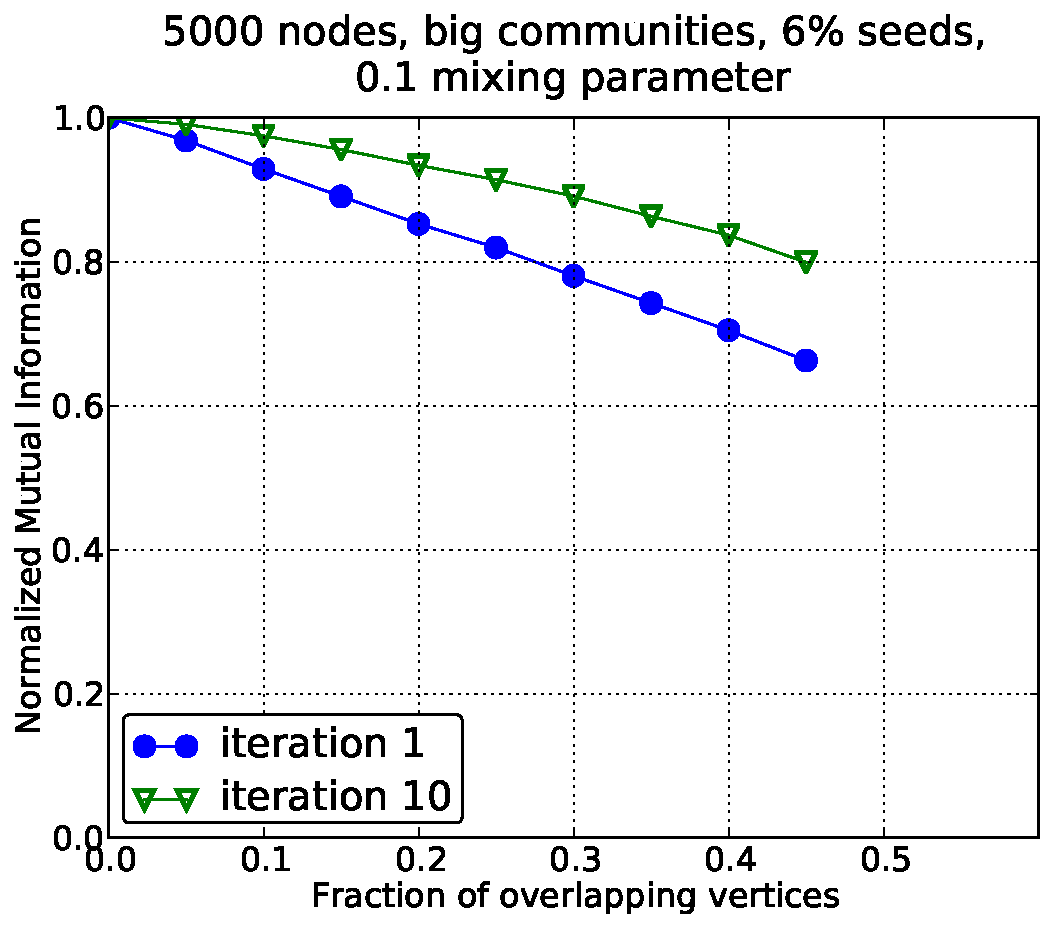
\includegraphics[width=\plotwidth]{plots/overlap_compare_b.pdf}
    \end{subfigure}
    \caption{Comparison between the the iterative and non-iterative method for overlapping communities.}\label{fig:compare_iter_overlap}
\end{figure}
%
\begin{figure}[h!]
    \centering
    \begin{subfigure}{0.4\textwidth}
    \centering
    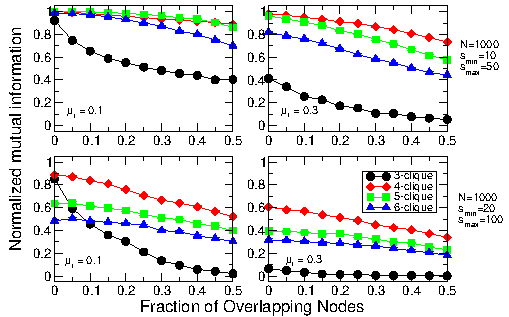
\includegraphics[width=\cfinderwidth]{lfrpaper/fig6.pdf}
    \end{subfigure}%
    \begin{subfigure}{0.4\textwidth}
    \centering
    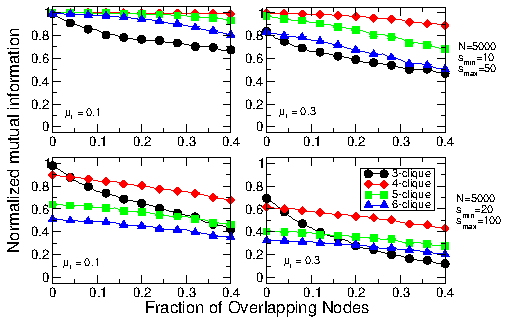
\includegraphics[width=\cfinderwidth]{lfrpaper/fig7.pdf}
    \end{subfigure}%
    \caption{
        Plots for CFinder on the LFR benchmark on graphs with 1000 and 5000 nodes 
		with overlapping communities. These figures are taken from~\cite{LF09}.
    }
\end{figure}


